\subsubsection{Introduction to $\gamma\gamma$ Colliders}
Photon colliders were originally proposed as potential extensions to linear colliders (there have been designs based on the ILC and CLIC\cite{CLIC:Multilinear}) but can also be built as independent machines. A photon collider operates using the process of inverse Compton scattering\textemdash generating  high energy gamma rays for colliding by directing a low energy laser beam ($\sim$1 eV) into a high energy electron beam (10s of GeV) i.e. the electrons transfer some of their energy to the photons\cite{Chou:Higgs}.

Gamma-gamma ($\gamma\gamma$) collisions result in a large cross section of $\gamma\gamma$ $\rightarrow$ H interactions similar to that in electron-positron colliders, e$^{+}$e$^{-}$ $\rightarrow$ ZH ($\sim$200 fb)\cite{Chou:Higgs} however the energy required for $\gamma\gamma$ collisions is a lot lower\textemdash 80 GeV electron beam energy compared to 120 GeV in the e$^{+}$e$^{-}$ colliders. This reduced energy requirement is beneficial to circular colliders as it corresponds to a decrease in the synchrotron radiation power by a factor of 5 and makes the option of building a circular photon collider at Fermilab named HFiTT\textemdash Higgs Factory in Tevatron Tunnel\textemdash a possibility\cite{Chou:Higgs}. 

The lower energy required for Higgs production makes photon colliders a good option for a new low energy, cost effective Higgs factory. Additional advantages of photon colliders include: no positron source is required, no damping rings, the high polarisation of photons and electrons and the ability to reuse existing infrastructure or extending ones that would be built anyway. However the physics capability of a photon collider is not as wide-ranging as a 240 GeV e$^{+}$e$^{-}$ collider and there are design issues to overcome such as IR optics, power consumption and removal of the spent electrons\cite{Blondel:HiggsF}.
 
\subsubsection{Physics of $\gamma\gamma$-to-Higgs}
A large cross-section of 200 fb is achieved in the direct s-channel $\gamma\gamma$ $\rightarrow$ H reaction. This is an important reaction and enhancement of the signal over the background is achieved for photons of circular polarization in the J=0 state by using a polarized laser\cite{Blondel:HiggsF}.  The CP properties of the Higgs Boson can be measured directly using linearly polarized high-energy photons. In fact photon colliders are the only machines capable of measuring the CP admixture and violation of the Higgs to an accuracy of 1\% or more\cite{Chou:Higgs}.

Photon colliders can measure the H-to-$\gamma\gamma$ partial width ($\gamma\gamma$) to a precision of 1\%\cite{Chou:Higgs}, which is better than any other collider. The $\gamma\gamma$ determines the production rate of Higgs in $\gamma\gamma$ collisions and can be measured by observing the decay mode H $\rightarrow$ bb accounting for ∼57\% of total Higgs decays. In e$^{+}$e$^{-}$− collisions, $\gamma\gamma$ is measured in the H $\rightarrow$ $\gamma\gamma$ decay which has a branching fraction of 0.24\%. Therefore at the photon collider, ``the statistics for the measurement of $\Gamma$(H $\rightarrow$ $\gamma\gamma$) is higher by a factor of $\frac{\frac{0.57}{0.0024}}{4}$ $\simeq$ 60 (and will be even larger if a lower-emmittance electron source becomes available).''\cite{Telnov:Photons} The H-to-$\gamma\gamma$ partial width is an important quantity in Higgs physics because the decay proceeds via an inclusive loop that could reveal heavier particles which the Higgs is unable to directly decay into\textemdash new physics potential.

\subsubsection{SAPPHiRE proposal}
SAPPHiRE (Small Accelerator for Photon-Photon Higgs Production using Recirculating Electrons) is a proposed stand-alone $\gamma\gamma$ collider that presents a cost and time efficient option for a Higgs factory capable of accurately measuring Higgs particle properties. The basic principle of operation in SAPPHiRE is based on the process of inverse compton scattering described above with the collider hitting accelerated electrons with a low energy laser beam ($\sim$3.5 eV) generating a back-scattered gamma beam for collision. By colliding photons, the limits to luminosity arising from beam-beam interactions (beamsstrahlung) of charged particles are avoided\cite{Zimmermann:SAPPHiRE}. The SAPPHiRE collider will be about 9Km in circumference and accelerate particles to 80 GeV thus making it the lowest-energy Higgs factory\cite{Bogacz:SAPPHiRE}.

\subsubsection{Technical design and parameters}                                                                                                            SAPPHIRE's design is based on a pair of $\sim$10 GeV recirculating Linacs, similar to those used for LHeC (the sapphire project emanated from the recirculating linac system at LHEC ). The collider has a Laser back scattering system able to produce a $\gamma\gamma$ peak luminosity of 0.36 × 1034 cm−2 s−1 with ECM ($\gamma\gamma$) ∼ 125 GeV. Hence it will be able to produce tens of thousands of Higgs (H) particles a year in clean experimental conditions\cite{Bogacz:SAPPHiRE}.

\begin{figure}
\centering
%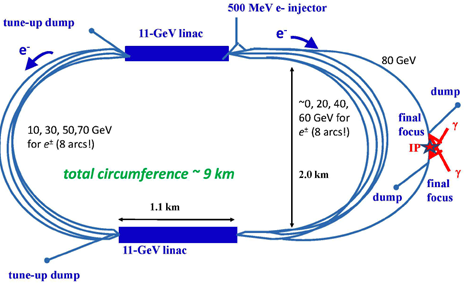
\includegraphics{sapphire1.png}
\caption{Schematic of the SAPPHiRE design based on recirculating superconducting linacs\cite{Bogacz:SAPPHiRE}.}
\end{figure}

The 80 GeV electron beam centre of mass energy required is reached by four passes through the two superconducting recirculating LINACs which increase the electron energy by $\sim$10GeV in each passing.  In comparison to the LHeC, an additional arc is required on both sides with respective beam energies of 70GeV and 80 GeV. The $\gamma\gamma$ collision point is located at the centre of the 80 GeV arc. The Compton scattering point (where gamma beams are generated) is to be located $\sim$1mm from the $\gamma\gamma$ interaction point and laser pulses are required at a frequency of 200kHz. The other laser parameters are: a wavelength of 351nm, 5J pulse energy and a long pulse duration of 5 ps\cite{Bogacz:SAPPHiRE}.

\begin{table}
\begin{center}
\begin{tabular}{l r}
\hline
\hline
Total electric power & 100 MW\\
Beam energy & 80 GeV\\
Beam polarization & 0.80\\
Beam population & $10^{10}$\\
\# of bunches per train & \textemdash\\
\# of trains per rf tube & \textemdash\\
Repetition rate & cw\\
Average bunch frequency & 200 kHz\\
Average beam current & 0.32 mA\\
RMS bunch length & 30 \textmu m\\
Crossing angle & $\geq$ 20mrad\\
Normalised horizontal emittance & 5 \textmu m\\
Nominal horizontal beta function at the IP & 0.5 \textmu m\\
Nominal vertical beta function at the IP & 5 mm\\
Nominal RMS horizontal IP spot size & 400 nm\\
Nominal RMS vertical IP spot size & 18 nm\\
Nominal RMS horizontal CP spot size & 400 nm\\
Nominal RMS vertical CP spot size & 180 nm\\
e$^{-}$e$^{-}$ geometric luminosity & $2.2 \times 10^{34} cm^{-2}s^{-1}$\\
\hline
\hline
\end{tabular}
\caption{Parameters for SAPPHiRE optimised for Higgs mass $\sim$125 GeV}
\end{center}
\end{table}

\subsubsection{Technical feasibility}
The energy loss in an arc is given by:

\begin{equation}
E_{arc}[GeV]=8.846 \times 10^{-5}\frac{(E \ [GeV])^{4}}{2\rho \ [m]}
\end{equation}

Where the bending radius, $\rho$ = 764 m (equal to the LHeC design) and the energy loss in each arc is shown in table 2. Each electron beam loses about 4 GeV in energy, which can be is compensated for by increasing the voltages of the two LINACs from 10 GV to 10.63 GV. The beams in the 70GeV arc lose the most energy due to synchrotron radiation: 1.39 GeV, or a 2\% loss\cite{Bogacz:SAPPHiRE}.

\begin{table}
\begin{center}
\begin{tabular}{c c c}
\hline
\hline
beam energy [GeV] & $\Delta E_{arc}$ [GeV] & $\Delta\sigma_{E}$ [MeV]\\
\hline
10 & 0.0006 & 0.038\\
20 & 0.009 & 0.43\\
30 & 0.05 & 1.7\\
40 & 0.15 & 5.0\\
50 & 0.36 & 10\\
60 & 0.75 & 20\\
70 & 1.39 & 35\\
80 & 1.19 & 27\\
\hline
total & 3.89 & 57 (0.071\%)\\
\hline
\hline
\end{tabular}
\caption{displays the energy losses and energy spread induced in the 8 arcs of SAPPHiRE}
\end{center}
\end{table}

The energy spread from synchrotron radiation in the arc bends is given by:
\begin{equation}
\Delta\sigma^{2}_{E}=\frac{\alpha(\hbar c)^{2}}{48\sqrt{3}}\gamma^{7}\frac{\pi}{\rho^{2}}
\end{equation}

With the geometric radius, R $\simeq$ 1 km and $\rho$ is the dipole bending radius in the arc. The total additional energy spread as a result of synchrotron radiation is only 0.071\%\cite{Bogacz:SAPPHiRE}.

The horizontal emmittance growth of the electron beam caused by synchrotron radiation poses a severe feasibility limitation and is given by:

\begin{equation}
\Delta_{\epsilon/N}=\frac{2pi}{3}\frac{c_{q}r_{e}}{\rho^{2}}\gamma^{6}\langle H \rangle
\end{equation}

Sapphire needs a smaller horizontal emmittance growth than the LHeC which has  = 13 microns at 60GeV.  Reducing the cell length and associated dipole length by a factor of 4 will reduce  at 80GeV to 1 micron, adequate for SAPPHiRE. This means the total length of the bending magnets per optical cell is reduced from $l_{bend}$ $\simeq$ 40 m in the LHeC design to $l_{bend}$ = 10 m for SAPPHiRE\cite{Bogacz:SAPPHiRE}.

Sapphire requires an emmittance ratio of $\frac{\epsilon_{x}}{\epsilon_{y}} \sim 10$, a bunch charge of 1.6 nC and an initial emmittance of $\sim$1.5 \textmu m. These parameters are achievable within the present state of the art. Hence the SAPPHiRE concept employs feasible accelerator parameters. However the main concern is whether we can get polarized beams with these parameters: a polarized low emmittance electron gun is needed. There are ongoing R \& D efforts looking into ``low-emmittance DC guns'' and ``polarized SRF guns.''\cite{Zimmermann:SAPPHiRE}

\subsubsection{Advantages of Sapphire}                                                                                                              The lower beam energy of 80 GeV required to create the Higgs boson allows for efficient recirculation and a 10 times smaller Radio Frequency installation (reducing costs)\cite{Bogacz:SAPPHiRE}. For a stand-alone collider such as the Sapphire, there is no positron beam requirement and no damping rings– further large savings and simplification.

High polarization in the primary electron and the colliding $\gamma$ beams\textemdash in contrast to the case of e$^{+}$\textemdash is becoming a possibility as the Laser technology needed to generate such beams is becoming a reality. SAPPHiRE designs are cost effective (\textless \$1 billion) and take advantage of existing technology and infrastructure. The photon collider concept is applicable to ILC/CLIC as a companion capability. There is no beamstrahlung which results in a higher energy reach than electron positron colliders\cite{Zimmermann:SAPPHiRE}.

\subsubsection{Main issues}
The major design limitation of the SAPPHiRE is the unacceptable increase of horizontal emmittance in the bending arcs: The authors of SAPPHiRE solve this by reducing the dipole section length by 4 which will result in a 64 times smaller emmittance dilution however this requires 16 times stronger quadrupole magnets (quads gradient will be 16 times larger)\cite{Telnov:Photons}.

The initial normalized beam emittances quoted in the sapphire paper of 5 μm and 0.5 μm in the x and y directions respectively, correspond to best unpolarised RF gun emittances but photon colliders need polarised electrons. Currently no low emittance polarized RF guns exist (though progress is being made)\cite{Telnov:Photons:MIT}.

The high-performance laser backscattering system required in collider requires the most R \& D, though money is likely to be made from spin-offs as a result of developments in laser systems which will be beneficial in other fields of science and industry. The main problem is in achieving the lasers high repetition rate of 200kHz; it is possible to overcome this using a passive optical cavity however this is very complex. An alternative approach involves the use of a free electron laser which is cheaper and less complex\cite{Zimmermann:TLEP}.

\subsubsection{Goals and summary of possible measurements}
SAPPHiRE can measure accurately the mass, bb, WW*, and $\gamma\gamma$ decays of the Higgs boson with corresponding plausible statistical errors on these decay paths of 2\%, 5\% and 8\% respectively. In addition, the Higgs mass can be measured to a predicted accuracy of $\sim$100 MeV after 2 years of operation. Other possible decay modes that should be observable include h $\rightarrow$ ZZ* and H $\rightarrow$ Z$\gamma$ but no studies have been made yet. Also, there is the possibility of observing H $\rightarrow$ $\tau^{+}\tau^{-}$ decay\cite{Bogacz:SAPPHiRE}.

CP properties of the H $\rightarrow$ $\gamma\gamma$ partial width can be measured with a precision of about 1\% by taking advantage of both linear and circular polarization, which can't be done at any other collider\cite{Chou:Higgs}.This quantity is of particular interest because the decay proceeds through an inclusive loop that has the potential to reveal heavier charged particles that the Higgs can't directly decay into. The high precision measurements of couplings to standard model particles and possible measurements of non-standard Higgs decays available at SAPPHiRE are beyond the scope of LHC.

\subsubsection{Location and cost}
SAPPHiRE is developed at CERN but could be built elsewhere: it could ``fit" on the SLAC site. Stand-alone photon colliders are compact machines that can be built using existing infrastructure. For example the proposed HFiTT would be located at Fermilab\cite{Chou:Higgs}. It could also be built or as a companion to linear accelerators such as ILC or CLIC. SAPPHIRE's estimated cost $\sim$\$1 billion\textemdash a small fraction of other future projects budgets. 

\subsubsection{Timeline}
Design reports for SAPPHiRE and other proposed photon colliders have not yet been produced. First a conceptual design report will need to be produced followed by a technical design report. 
Taking into account technical readiness, if a stand-alone $\gamma\gamma$ collider such as Sapphire is to be built, it is likely (on a CERN time-scale) to start construction in 2022 with the completion of 5 years of its experimental programme estimated to be sometime between 2030 and 2035. On the other hand if built as an add-on to a linear collider, it would be operational within the active life of e.g. the ILC (2030-2045)\cite{Blondel:HiggsF}.

\subsubsection{Spin-offs}
The generated high energy photon beams have the following characteristics: bright source, monochromatic scattered light (after collimation), tunable wavelength, less expensive than XFEL, broad energy reach (keV, MeV, GeV, TeV) and polarization. Applications of these properties include medical purposes, nuclear material detection and for obtaining polarised e$^{+}$ for e$^{+}$e$^{-}$ linear colliders and many more\cite{Telnov:Overview}.

Spin-offs are likely to be made from the R \& D necessary to create the high-performance laser backscattering system and the polarized RF guns that will be useful in other fields of basic science and industry.

\subsubsection{Conclusion}
SAPPHiRE provides a time and cost effective choice for a Higgs factory. SAPPHiRE can produce the same order of Higgs bosons as an e$^{+}$e$^{-}$ collider and has potential for CP studies and new physics discoveries. However a key issue is the unacceptable increase of the horizontal emittance in the bending arcs. Electron-positron linear colliders can study a greater range of Higgs properties so there is little chance that the physics community will support building SAPPHiRE as the next particle collider instead of e$^{+}$e$^{-}$, and so a photon collider such as SAPPHiRE is best built as an add-on to an e$^{+}$e$^{-}$  collider. Linear colliders are very expensive projects and should be built to maximise the discovery potential therefore considering the relatively low cost of adding a photon collider to a linear collider, a good solution is to combine the two into a collider with two interaction points.

Such an addition at the ILC is conceptually clear but requires enhanced technical design of the laser system. The main thing holding it back is the fact that photon linear colliders need polarized electrons (only in this case can you see the Higgs) and currently low emittance polarized electron guns do not exist.
